Для того чтобы показать, что задача является \textbf{NP трудной}, необходимо построить полиномиальную редукцию
для некоторой NP полной задачи, а так же показать что решение задачи позволяет получить решение некоторой
NP полной задачи.

Сначала введем некоторые определения.

% Как будто не понятно причем тут графы, нужно как-то пояснить что выбор кандидатов на спил
% и все остальное в данный момент нас не интерисует. То есть сейчас мы знаем что регистры можно распределить

\begin{definition}

    \label{def:liveness} % Мне все равно не очень нравится это определение

    Представим исходный код в виде CFG (control flow graph).
    Будем говорить что переменная $x$ \textit{жива} в точке $p$, если существует путь в CFG из точки определения, проходящий
    через $p$ и использование переменной, на котором не встречается другого определения переменной $x$.

\end{definition}

\begin{definition}

    Будем говорить что переменные $a$ и $b$ \textit{зацеплены}, если одна из переменных жива в точке объявления
    другой переменной.

\end{definition}

\begin{definition}

    $IG(V)$ -- \textit{граф зацепленности} для множества переменных некоторой программы.
    $IG(V) = (V, E)$, где $V$ -- множество переменных, а
    $$E = \{(a, b) \ | \  a, b \in V \land \ a \text{ и } b \text{ -- зацеплены}\}.$$

\end{definition}

Если удастся получить раскраску этого графа в n цветов, то и проблема распределения переменных по
n регистрам для этой программы будет решена.

Рассмотрим простой пример:

\begin{example}
    \begin{figure}[h]
        \centering
        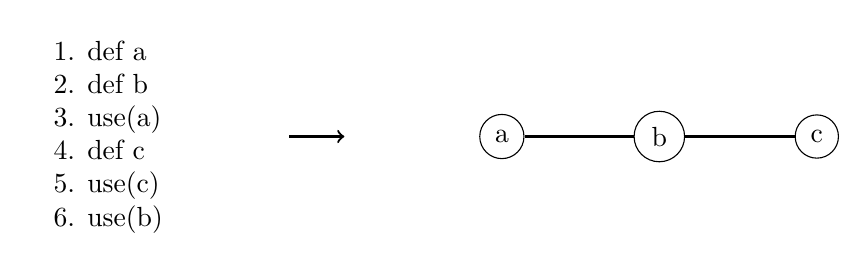
\begin{tikzpicture}
            \node at (0, 0) {\begin{tabular}{l}
                1. def a \\
                2. def b \\
                3. use(a)\\
                4. def c \\
                5. use(c)\\
                6. use(b)
            \end{tabular}};

            \draw[->, thick] (2.3, 0) -- (3, 0);
        
            \node[circle, draw] (a) at (5, 0) {a};
            \node[circle, draw] (b) at (7, 0) {b};
            \node[circle, draw] (c) at (9, 0) {c};
        
            \draw[thick] (a) -- (b);
            \draw[thick] (b) -- (c);
        \end{tikzpicture}
    \caption{Пример преобразования кода в граф}
    \begin{tabular}{r @{: } l}
        \textbf{def} & Объявление переменной \\
        \textbf{use} & Использование переменной \\
    \end{tabular}
    \label{fig:ex1}
    \end{figure}

    % \begin{figure}
    % \centering
    % \begin{tikzpicture}
    %     \node[circle, fill=cyan!60!white, draw] (a) at (5, 0) {a};
    %     \node[circle, fill=magenta!60!white, draw] (b) at (7, 0) {b};
    %     \node[circle, fill=cyan!60!white, draw] (c) at (9, 0) {c};
        
    %     \draw[thick] (a) -- (b);
    %     \draw[thick] (b) -- (c);

    % \end{tikzpicture}
    % \caption{Раскрашенный граф}
    % \label{fig:ex1-color}
    % \end{figure}

    В графе на рисунке~\ref{fig:ex1} есть ребро $(a, b)$ потому что в точке 2 переменная $a$ \textit{жива}, но в графе нет ребра $(a, c)$
    потому что в момент 4 у переменной $a$ не найдется пути который прошел бы через использование.
    
\end{example}

Теперь покажем, что по заданному графу можно построить программу, распределение регистров которой даст раскраску.

Пусть $\text{Var}$ -- множество переменных, $\text{R}$ -- множество регистров.
Тогда пусть существует отображение $\varphi : \text{Var} \to R$. При этом выполняются следующее свойство:

$$\forall a, b \in \text{Var} \text{ a и b интерферируют}  \Rightarrow \varphi(a) \neq \varphi(b)$$

Если построить биективное отображение $\psi: R \to C$, где множество $C$ -- множество цветов.
То раскраска графа $IG(V)$ строится как $\zeta = \psi \circ \varphi$.

% Мысль закончилась

В своей статье Чайтин~\cite{chaitin1982} предложил следующий алгоритм построения кода из графа:

\begin{enumerate}
    \item Если в графе существует вершина $\text{NODE}_i$, то в исходном коде будет объявление переменной с таким
    названием.
    \item Если в графе есть ребро $(\text{NODE}_i, \text{NODE}_j)$, то в исходном коде добавим использование переменных
    например суммирование. Так, чтобы эти переменные не могли занимать один регистр.
\end{enumerate}

Этот метод работает не всегда. Иногда требуются дополнительные конструкции например \textit{операторы ветвления},
для того чтобы проблема раскраски графа действительно свилась к проблеме распределения регистров. Рассмотрим пример когда такие
преобразования потребуются.

\begin{example}

    \begin{figure}[h]
        \centering
        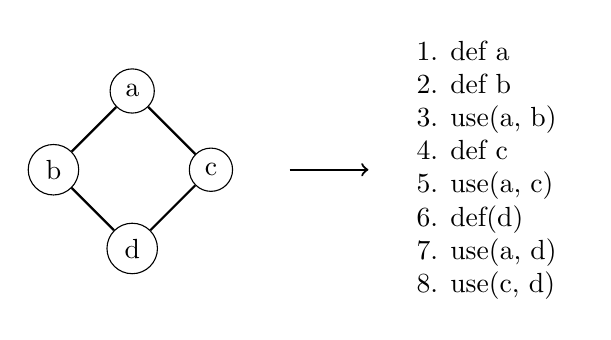
\begin{tikzpicture}
            \node at (6.5, 0) {\begin{tabular}{l}
                1. def a \\
                2. def b \\
                3. use(a, b) \\
                4. def c \\
                5. use(a, c) \\
                6. def(d) \\
                7. use(a, d) \\
                8. use(c, d)
            \end{tabular}};

            \draw[->, thick] (4, 0) -- (5, 0);
        
            \node[circle, draw] (a) at (2, 1) {a};
            \node[circle, draw] (b) at (1, 0) {b};
            \node[circle, draw] (c) at (3, 0) {c};
            \node[circle, draw] (d) at (2, -1) {d};
        
            \draw[thick] (a) -- (b);
            \draw[thick] (a) -- (c);
            \draw[thick] (b) -- (d);
            \draw[thick] (c) -- (d);
        \end{tikzpicture}
    \caption{Пример преобразования графа в код}
    \label{fig:ex2}
    \end{figure}

    На рисунке~\ref{fig:ex2} видно, что код построенный по алгоритму который был предложен Чайтином не
    всегда соответствует изначальному графу. В этом случае в исходном коде переменные
    $a$ и $d$ интерферируют, хотя в изначальном графе ребра $(a, d)$ не было. Код построенный
    по графу из рисунка~\ref{fig:ex2} должен выглядеть как на рисунке~\ref{fig:right_ex2}.

    \begin{figure}
        \centering
        \lstset{basicstyle=\ttfamily\small, frame=single}
        \begin{lstlisting}
            01. def a
            02. if statement:
            03.     def b
            04.     use(a)
            05.     def d 
            06. else:
            07.     def c
            08.     use(a)
            09.     def d
            10. use(d)
        \end{lstlisting}
        \caption{Правильный вид исходного кода}
        \label{fig:right_ex2}
    \end{figure}
\end{example}

Алгоритм Чайтина легко исправляется следующим подходом: (Алгоритм под вопросом)

\begin{enumerate} %% ??
    \item Для каждой вершины исходного графа создать переменную.
    \item Если между вершинами существует ребро, то создать \texttt{if statement}, в теле
    которого объявить эти переменные и использовать таким образом, чтобы они стали зацеплены.
\end{enumerate}